\documentclass{beamer}
\usepackage[T1]{fontenc}
\usepackage[utf8]{inputenc}
\usepackage{lmodern}
\usepackage[brazil]{babel}
\usepackage[labelformat=empty]{caption}
\usepackage{graphicx}
\usepackage{color}

\definecolor{beamer@blendedblue}{rgb}{0.5, 0.6, 0.4}
\definecolor{covered}{gray}{0.65}
\definecolor{filecolor}{rgb}{0, 0.3, 0.7}
\usetheme{Warsaw}
\title[NetSim: um simulador de redes simplificado.]{NetSim: um simulador de redes simplificado.}
\author{Carlos Eduardo Leão Elmadjian \and Renan Fichberg}
\date{11 de novembro de 2014}
\institute{Instituto de Matemática e Estatística da Universidade de São Paulo (IME-USP)}

\expandafter\def\expandafter\insertshorttitle\expandafter{%
\insertshorttitle\hfill%
\insertframenumber\,/\,\inserttotalframenumber}

\begin{document}

\begin{frame}
	\titlepage
\end{frame}

\begin{frame}
\begin{center}
	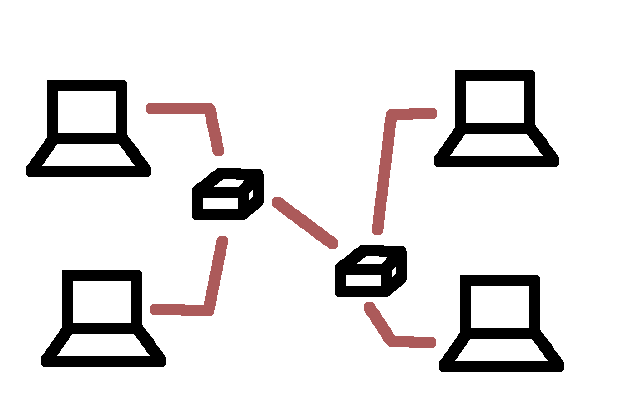
\includegraphics[scale=0.4]{simulator.png}
\end{center}
\end{frame}

\begin{frame}
	\frametitle{Conteúdo}
	\begin{itemize}
		\item O simulador: como funciona
		\item Testes realizados com o simulador
		\item Dificuldades encontradas
	\end{itemize}
\end{frame}

\end{document}